\chapter{Vervolg}
\label{ch:vervolg}

In dit hoofdstuk zal er beschreven worden wat het vervolg kan zijn van deze bachelorproef. Hoe kunnen anderen aan de programmeercode geraken, hoe kunnen anderen de website raadplegen of hoe kan de \textit{webserver} geïnstalleerd worden binnen het HoGent-netwerk.

\section{Applicatie-code delen}
Om er zeker van te zijn dat deze bachelorproef niet onder het stof verdwijnt en dat de applicatie niet meer gebruikt zal worden is het noodzakelijk dat de volledige programmacode gedeeld kan worden. Hiervoor zal er gebruik gemaakt worden van ``GitHub''.

Om GitHub te begrijpen is het eerst nodig wat Git zelf is. Git is een open source versiebeheersysteem. Wanneer ontwikkelaars iets maken of programmeren brengen ze wijzigingen aan in de code waarbij er nieuwe versies uitkomen. Versiebeheersystemen beheren deze revisies door alle wijzigingen op te slaan in een centrale opslagplaats. Hierdoor kunnen ontwikkelaars gemakkelijk samenwerken, omdat ze een nieuwe versie van de software kunnen downloaden, wijzigen en zelf nieuwe revisies kunnen uploaden. Elke programmeur van de project kan dan op zijn of haar beurt weer zien welke wijzigingen er doorgevoerd zijn en kan deze opnieuw downloaden.~\autocite{Brown2019}

GitHub is dus zo een voorbeeld van een centrale opslagplaats plaats waar alle wijzigingen opgeslagen staan in de \textit{cloud}.

Alle code, bestanden en revisies van deze volledige bachelorproef zijn dan ook te vinden op de volgende URL: ``\url{https://github.com/SibianDG/BachelorProef}'' met de nodige toestemmingen.

\section{Hosting- Bereikbaarheid van de applicatie}
Om te kunnen spreken hoe we het beste de applicatie beschikbaar maken is het eerst noodzakelijk dat iedereen weet wat dat allemaal betekent.

De huidige opstelling van dit eindwerk is geïllustreerd in figuur \ref{fig:opstelling_bachelorproef}. Daarbij is alle code geïnstalleerd, of eerder gezegd aanwezig op die lokale computer zelf. Wanneer er het bestand `website.py' wordt uitgevoerd zal Python de code uitvoeren en een webserver opzetten op die lokale machine. In de output verschijnt er dan een website-adres. Als er naar de website gegaan wordt ziet u de applicatie.

\begin{figure}
    \centering
    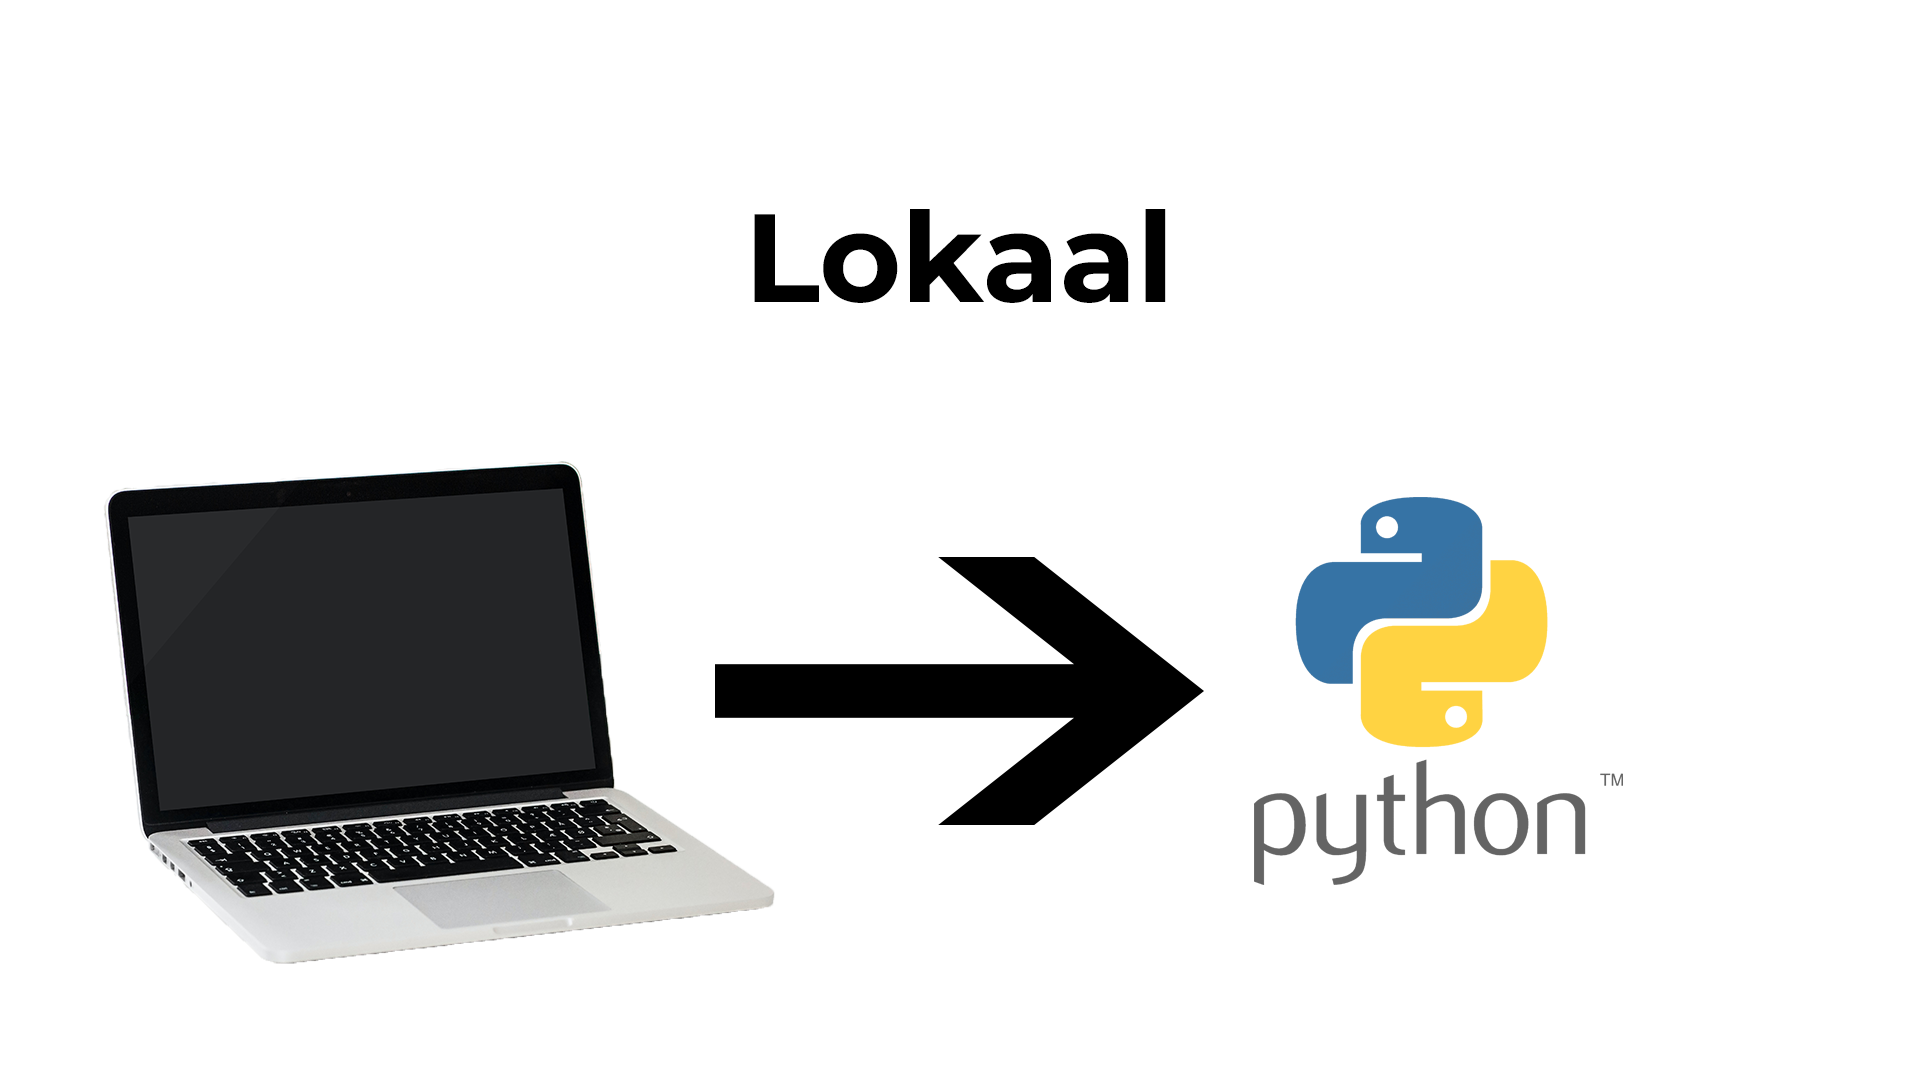
\includegraphics[width=1\textwidth]{./img/lokaal_website}
    \caption{\label{fig:opstelling_bachelorproef} Opstelling bachelorproef}
\end{figure}

Wanneer we de website beschikbaar willen maken voor meerdere computers moeten we de code op een server installeren. Zo kunnen er meerde \textit{clients} een aanvraag of \textit{request} sturen naar de server die alles afhandelt zoals de webpagina tonen en de berekeningen uitvoeren. Een illustratie is te vinden op figuur \ref{fig:webhosting_scheme}. Daarbij is te zien dat wanneer een gebruiker of \textit{user} naar een website surft, er een verzoek verstuurd wordt naar het internet. Het internet weet op zijn beurt aan welke webserver die informatie kan vragen of sturen. De server zelf handelt de website zelf af, de \textit{html}-, en javascriptpagina's als websitebestanden, en doet ook de berekeningen.

\begin{figure}
    \centering
    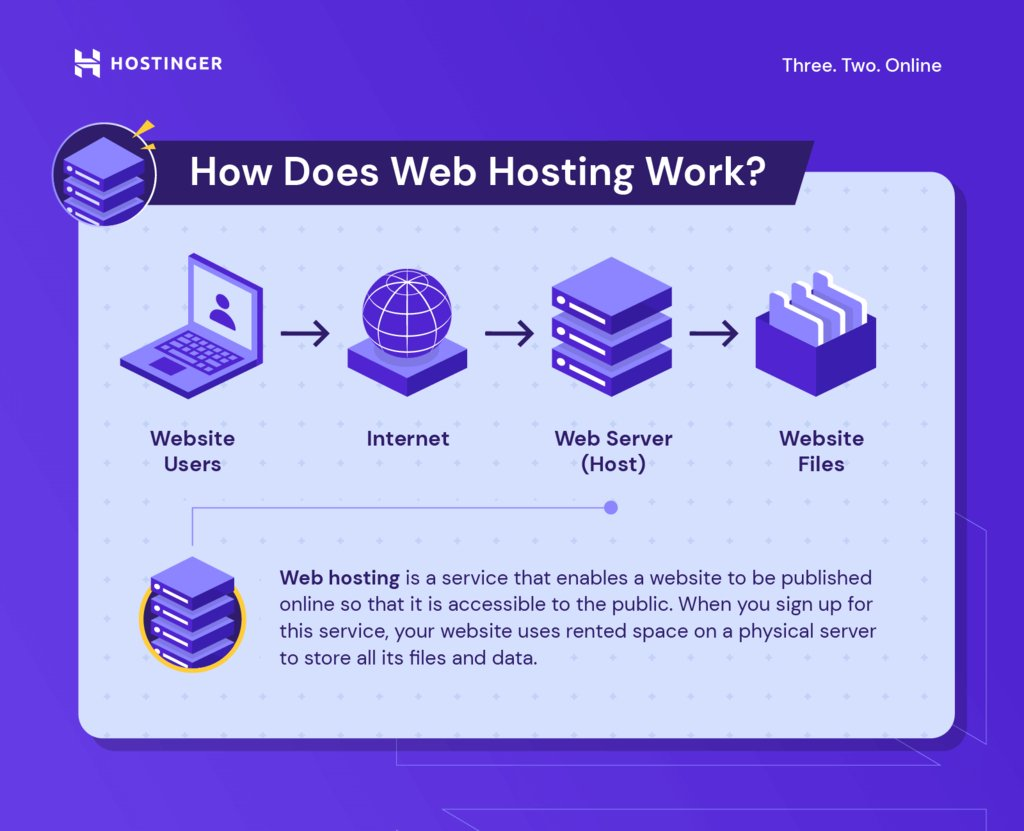
\includegraphics[width=1\textwidth]{./img/how-does-web-hosting-work}
    \caption{\label{fig:webhosting_scheme} Hoe werkt webhosting.~\autocite{Tamara2022}}
\end{figure}

\subsection{Installeren op een computer}
Hoe kan men alles installeren op een enkele computer?
In de hoofdmap met alle code is er een bestand te vinden genaamd ``requirements.txt''. Door het commando:
\begin{python}
    pip install -r requirements.txt
\end{python}
uit te voeren zullen alle Python-bibliotheken geïnstalleerd worden die nodig zijn om het project uit te voeren. Op Windows moet er wel nog een extra stap gebeuren en dat is FFmpeg apart installeren. De stappen daarvan staan beschreven op de volgende website: ``\url{https://www.wikihow.com/Install-FFmpeg-on-Windows}''.
\subsubsection{Mogelijkheden}
\begin{itemize}
    \item Snelle opzet voor IT'ers
    \item Snelle verwerking omdat het op dezelfde computer gebeurt en er maar 1 persoon aan kan
\end{itemize}
\subsubsection{Beperkingen}
\begin{itemize}
    \item Andere computers hebben geen toegang
    \item Niet-IT'ers kunnen het mogelijks minder makkelijk installeren
    \item Alles zou geïnstalleerd moeten worden op elke computer opnieuw
\end{itemize}

\subsection{Hosten in een lokaal netwerk}
Het is ook mogelijk om de software op een computer te installeren, deze te laten aan staan, maar met een speciale parameter. Wanneer er in de Flask-applicatie de volgende parameter wordt meegegeven: ``host='0.0.0.0''. Hierdoor zal de applicatie opengesteld worden in het lokale netwerk. Dit laat het mogelijk naar het lokale IP-adres de surfen op een ander toestel en ook de detector te kunnen gebruiken.
\subsubsection{Mogelijkheden}
\begin{itemize}
    \item Een keer installeren op een computer van bijvoorbeeld de docent in kwestie, en nadien kan het programma altijd opgestart worden tijdens een les.
    \item Een gratis oplossing
    \item Meerdere connecties mogelijk
\end{itemize}
\subsubsection{Beperkingen}
\begin{itemize}
    \item Het maximale aantal connecties is afhankelijk van de computer waar de applicatie wordt opgestart. Hoe beter en sneller de computer, hoe meer connecties mogelijk en hoe sneller.
\end{itemize}

\subsection{Gratis hosting online}
Heroku
\subsubsection{Mogelijkheden}
\subsubsection{Beperkingen}

\section{Testen}
De testen die verzameld zijn is niet van een bijzonder grote grootteorde. Er kunnen extra testengevallen opgenomen worden in een vervolgopdracht. Dit kan een interdisciplinaire opdracht zijn met de richting verpleegkunde of communicatie. Hoe meer testen, hoe correcter het percentage dat aangeeft hoe goed de applicatie werkt.

Een opdracht bij de richting verpleegkunde kan het volgende zijn: de studenten maken en/of klasseren audio-opnames van eventuele \textit{elderspeak}. Hierna kan de gelabelde data gevoed worden aan het Python-script dat er geschreven is voor deze bachelorproef. Hierna kan er achterhaald worden hoe goed de applicatie presteert

In een richting van communicatie kan alle data opnieuw gelabeld worden, waar men veel kennis heeft rond dit fenomeen. Zo kan de data zeer nauwkeurig gelabeld worden, terwijl er in dit eindwerk de data gelabeld is door een persoon op basis van een persoonlijk mening...(TODO: zin herschrijven)
